% Standalone Architecture Diagrams for FarmFederate
% Compile with: pdflatex architectures.tex

\documentclass[border=10pt]{standalone}
\usepackage{tikz}
\usepackage{xcolor}
\usetikzlibrary{shapes,arrows,positioning,calc,fit,backgrounds,matrix,decorations.pathreplacing,shadows}

% Custom colors
\definecolor{llmcolor}{RGB}{65,105,225}
\definecolor{vitcolor}{RGB}{34,139,34}
\definecolor{vlmcolor}{RGB}{178,34,34}
\definecolor{fedcolor}{RGB}{255,140,0}
\definecolor{qdrantcolor}{RGB}{128,0,128}
\definecolor{inputcolor}{RGB}{70,130,180}
\definecolor{outputcolor}{RGB}{60,179,113}

\begin{document}

% ============================================================================
% FIGURE 1: Complete System Architecture
% ============================================================================
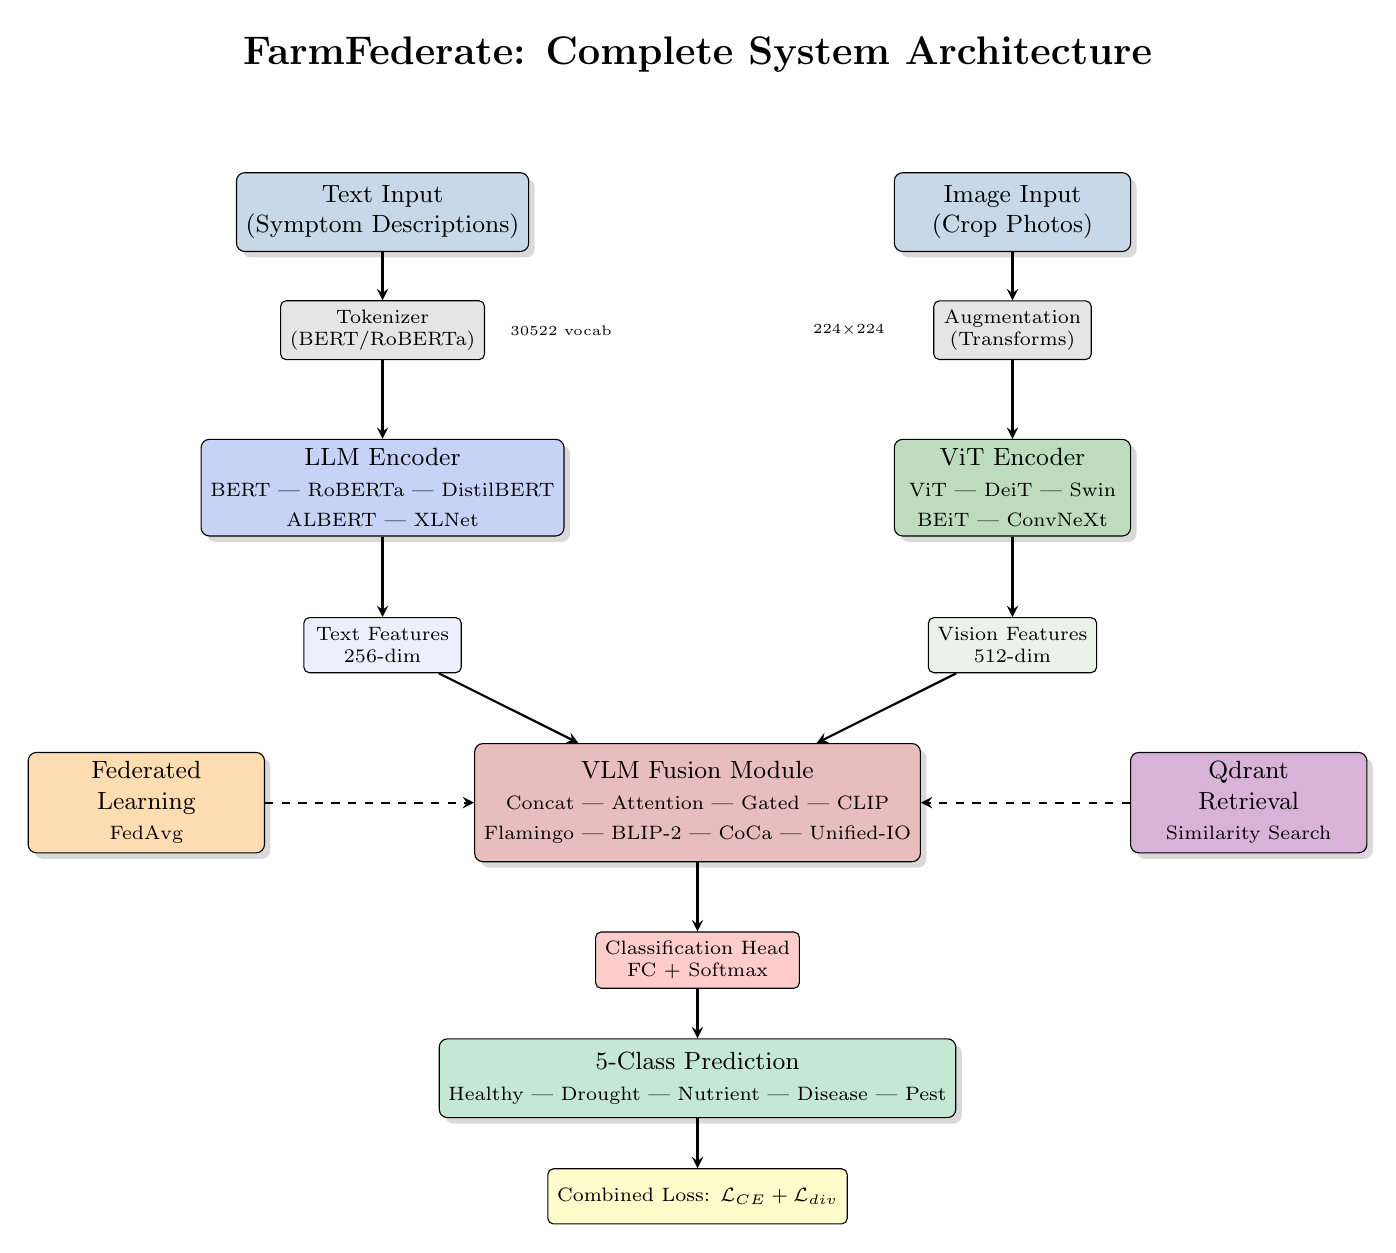
\begin{tikzpicture}[
    node distance=1.5cm,
    box/.style={
        rectangle, draw, rounded corners=3pt,
        minimum width=3cm, minimum height=1cm,
        align=center, font=\small,
        drop shadow={opacity=0.3}
    },
    smallbox/.style={
        rectangle, draw, rounded corners=2pt,
        minimum width=2cm, minimum height=0.7cm,
        align=center, font=\scriptsize
    },
    inputbox/.style={box, fill=inputcolor!30},
    llmbox/.style={box, fill=llmcolor!30},
    vitbox/.style={box, fill=vitcolor!30},
    vlmbox/.style={box, fill=vlmcolor!30},
    fedbox/.style={box, fill=fedcolor!30},
    dbbox/.style={box, fill=qdrantcolor!30},
    outputbox/.style={box, fill=outputcolor!30},
    arrow/.style={->, >=stealth, thick},
    dasharrow/.style={->, >=stealth, thick, dashed}
]

% Title
\node[font=\Large\bfseries] at (4, 5) {FarmFederate: Complete System Architecture};

% Input Layer
\node[inputbox] (text_in) at (0, 3) {Text Input\\(Symptom Descriptions)};
\node[inputbox] (img_in) at (8, 3) {Image Input\\(Crop Photos)};

% Preprocessing
\node[smallbox, fill=gray!20] (tokenizer) at (0, 1.5) {Tokenizer\\(BERT/RoBERTa)};
\node[smallbox, fill=gray!20] (augment) at (8, 1.5) {Augmentation\\(Transforms)};

% Encoders
\node[llmbox] (llm) at (0, -0.5) {LLM Encoder\\{\scriptsize BERT | RoBERTa | DistilBERT}\\{\scriptsize ALBERT | XLNet}};
\node[vitbox] (vit) at (8, -0.5) {ViT Encoder\\{\scriptsize ViT | DeiT | Swin}\\{\scriptsize BEiT | ConvNeXt}};

% Feature dimensions
\node[smallbox, fill=llmcolor!10] (text_feat) at (0, -2.5) {Text Features\\256-dim};
\node[smallbox, fill=vitcolor!10] (vis_feat) at (8, -2.5) {Vision Features\\512-dim};

% Fusion Module
\node[vlmbox, minimum width=5cm, minimum height=1.5cm] (fusion) at (4, -4.5) {
    VLM Fusion Module\\
    {\scriptsize Concat | Attention | Gated | CLIP}\\
    {\scriptsize Flamingo | BLIP-2 | CoCa | Unified-IO}
};

% Classifier
\node[smallbox, fill=red!20] (cls) at (4, -6.5) {Classification Head\\FC + Softmax};

% Output
\node[outputbox] (output) at (4, -8) {5-Class Prediction\\{\scriptsize Healthy | Drought | Nutrient | Disease | Pest}};

% Side modules
\node[fedbox] (fed) at (-3, -4.5) {Federated\\Learning\\{\scriptsize FedAvg}};
\node[dbbox] (qdrant) at (11, -4.5) {Qdrant\\Retrieval\\{\scriptsize Similarity Search}};

% Loss components
\node[smallbox, fill=yellow!20] (loss) at (4, -9.5) {Combined Loss: $\mathcal{L}_{CE} + \mathcal{L}_{div}$};

% Arrows - main flow
\draw[arrow] (text_in) -- (tokenizer);
\draw[arrow] (img_in) -- (augment);
\draw[arrow] (tokenizer) -- (llm);
\draw[arrow] (augment) -- (vit);
\draw[arrow] (llm) -- (text_feat);
\draw[arrow] (vit) -- (vis_feat);
\draw[arrow] (text_feat) -- (fusion);
\draw[arrow] (vis_feat) -- (fusion);
\draw[arrow] (fusion) -- (cls);
\draw[arrow] (cls) -- (output);
\draw[arrow] (output) -- (loss);

% Arrows - side modules
\draw[dasharrow] (fed) -- (fusion);
\draw[dasharrow] (qdrant) -- (fusion);

% Annotations
\node[font=\tiny, right] at (1.5, 1.5) {30522 vocab};
\node[font=\tiny, left] at (6.5, 1.5) {224$\times$224};

\end{tikzpicture}

\newpage

% ============================================================================
% FIGURE 2: LLM Architecture Detail
% ============================================================================
\begin{tikzpicture}[
    node distance=0.8cm,
    box/.style={rectangle, draw, rounded corners=2pt, minimum width=2cm, minimum height=0.6cm, align=center, font=\scriptsize},
    arrow/.style={->, >=stealth}
]

% Title
\node[font=\large\bfseries] at (5, 6) {Text Encoder (LLM) Architecture};

% Input
\node[box, fill=inputcolor!30] (input) at (0, 4.5) {Input Text\\``Leaves show wilting...''};

% Tokenizer
\node[box, fill=gray!20] (tok) at (0, 3) {Tokenizer\\[CLS] leaves show ...};

% Embedding
\node[box, fill=blue!20] (embed) at (0, 1.5) {Token Embedding\\30522 $\times$ 256};

% Position
\node[box, fill=yellow!20] (pos) at (0, 0) {+ Position Embedding\\max\_len $\times$ 256};

% Transformer blocks
\node[box, fill=llmcolor!30, minimum height=2cm] (trans) at (0, -2) {
    Transformer Encoder\\
    {\tiny Self-Attention}\\
    {\tiny Feed-Forward}\\
    {\tiny Layer Norm}
};

% Pooling
\node[box, fill=green!20] (pool) at (0, -4) {Adaptive Avg Pool\\+ Dropout (0.3)};

% Output
\node[box, fill=outputcolor!30] (out) at (0, -5.5) {256-dim Text Features};

% Arrows
\draw[arrow] (input) -- (tok);
\draw[arrow] (tok) -- (embed);
\draw[arrow] (embed) -- (pos);
\draw[arrow] (pos) -- (trans);
\draw[arrow] (trans) -- (pool);
\draw[arrow] (pool) -- (out);

% LLM variants on the right
\node[font=\small\bfseries] at (6, 4) {LLM Variants};

\node[box, fill=llmcolor!20] (bert) at (6, 2.5) {BERT\\110M params};
\node[box, fill=llmcolor!20] (roberta) at (6, 1.5) {RoBERTa\\125M params};
\node[box, fill=llmcolor!20] (distil) at (6, 0.5) {DistilBERT\\66M params};
\node[box, fill=llmcolor!20] (albert) at (6, -0.5) {ALBERT\\12M params};
\node[box, fill=llmcolor!20] (xlnet) at (6, -1.5) {XLNet\\110M params};

% Key features
\node[font=\tiny, align=left] at (9, 2.5) {Bidirectional};
\node[font=\tiny, align=left] at (9, 1.5) {Dynamic masking};
\node[font=\tiny, align=left] at (9, 0.5) {Distilled};
\node[font=\tiny, align=left] at (9, -0.5) {Parameter sharing};
\node[font=\tiny, align=left] at (9, -1.5) {Permutation LM};

\end{tikzpicture}

\newpage

% ============================================================================
% FIGURE 3: ViT Architecture Detail
% ============================================================================
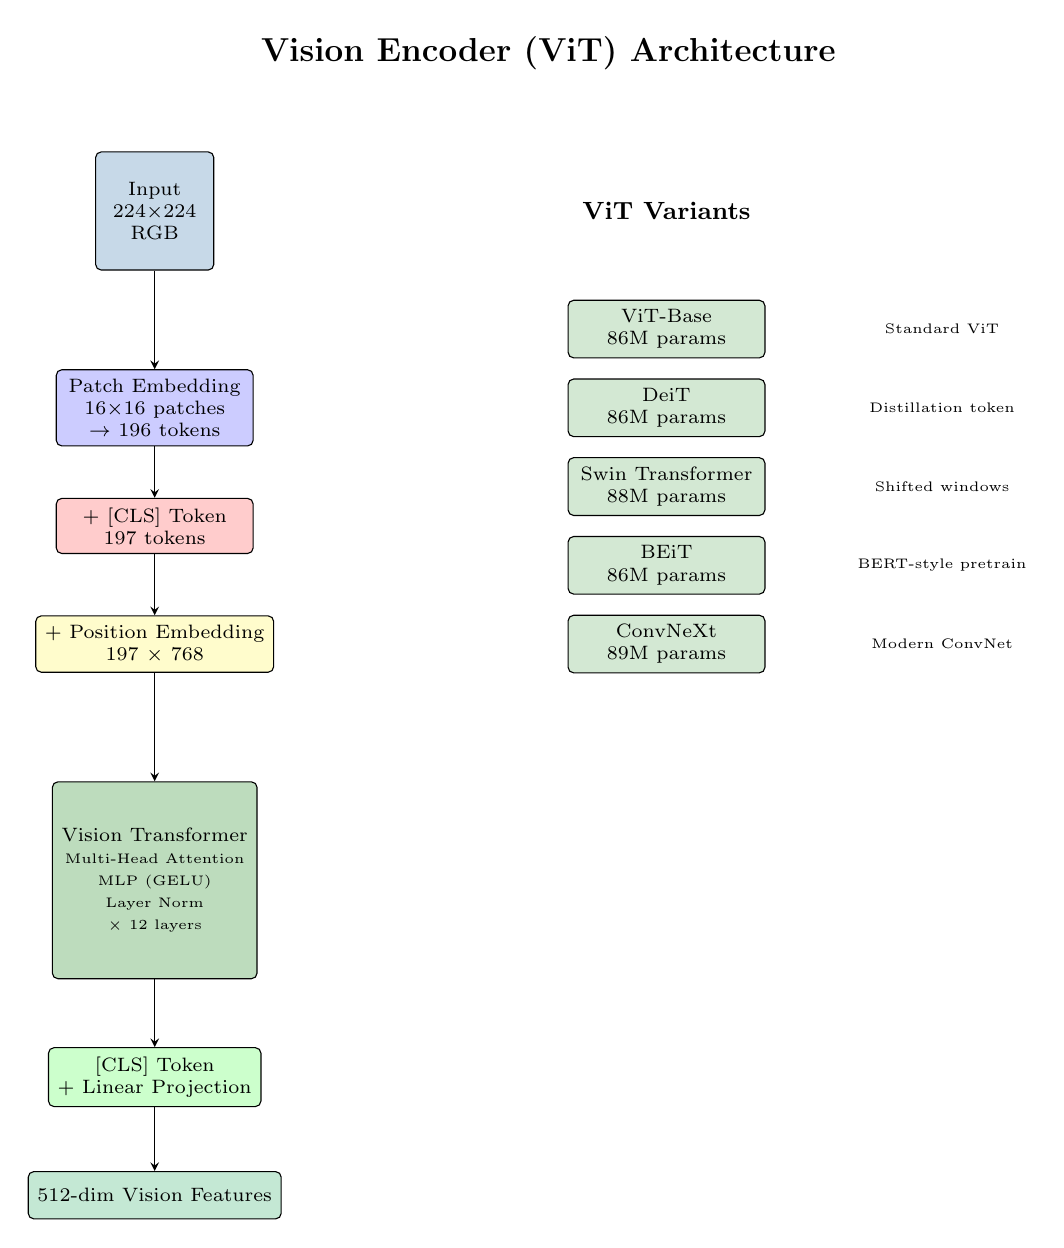
\begin{tikzpicture}[
    node distance=0.8cm,
    box/.style={rectangle, draw, rounded corners=2pt, minimum width=2.5cm, minimum height=0.6cm, align=center, font=\scriptsize},
    arrow/.style={->, >=stealth}
]

% Title
\node[font=\large\bfseries] at (5, 7) {Vision Encoder (ViT) Architecture};

% Input image
\node[box, fill=inputcolor!30, minimum width=1.5cm, minimum height=1.5cm] (img) at (0, 5) {Input\\224$\times$224\\RGB};

% Patch embedding
\node[box, fill=blue!20] (patch) at (0, 2.5) {Patch Embedding\\16$\times$16 patches\\$\rightarrow$ 196 tokens};

% CLS token
\node[box, fill=red!20] (cls) at (0, 1) {+ [CLS] Token\\197 tokens};

% Position embedding
\node[box, fill=yellow!20] (pos) at (0, -0.5) {+ Position Embedding\\197 $\times$ 768};

% Transformer
\node[box, fill=vitcolor!30, minimum height=2.5cm] (trans) at (0, -3.5) {
    Vision Transformer\\
    {\tiny Multi-Head Attention}\\
    {\tiny MLP (GELU)}\\
    {\tiny Layer Norm}\\
    {\tiny $\times$ 12 layers}
};

% Pool
\node[box, fill=green!20] (pool) at (0, -6) {[CLS] Token\\+ Linear Projection};

% Output
\node[box, fill=outputcolor!30] (out) at (0, -7.5) {512-dim Vision Features};

% Arrows
\draw[arrow] (img) -- (patch);
\draw[arrow] (patch) -- (cls);
\draw[arrow] (cls) -- (pos);
\draw[arrow] (pos) -- (trans);
\draw[arrow] (trans) -- (pool);
\draw[arrow] (pool) -- (out);

% ViT variants
\node[font=\small\bfseries] at (6.5, 5) {ViT Variants};

\node[box, fill=vitcolor!20] (vitbase) at (6.5, 3.5) {ViT-Base\\86M params};
\node[box, fill=vitcolor!20] (deit) at (6.5, 2.5) {DeiT\\86M params};
\node[box, fill=vitcolor!20] (swin) at (6.5, 1.5) {Swin Transformer\\88M params};
\node[box, fill=vitcolor!20] (beit) at (6.5, 0.5) {BEiT\\86M params};
\node[box, fill=vitcolor!20] (convnext) at (6.5, -0.5) {ConvNeXt\\89M params};

% Features
\node[font=\tiny, align=left] at (10, 3.5) {Standard ViT};
\node[font=\tiny, align=left] at (10, 2.5) {Distillation token};
\node[font=\tiny, align=left] at (10, 1.5) {Shifted windows};
\node[font=\tiny, align=left] at (10, 0.5) {BERT-style pretrain};
\node[font=\tiny, align=left] at (10, -0.5) {Modern ConvNet};

\end{tikzpicture}

\newpage

% ============================================================================
% FIGURE 4: All 8 VLM Fusion Architectures
% ============================================================================
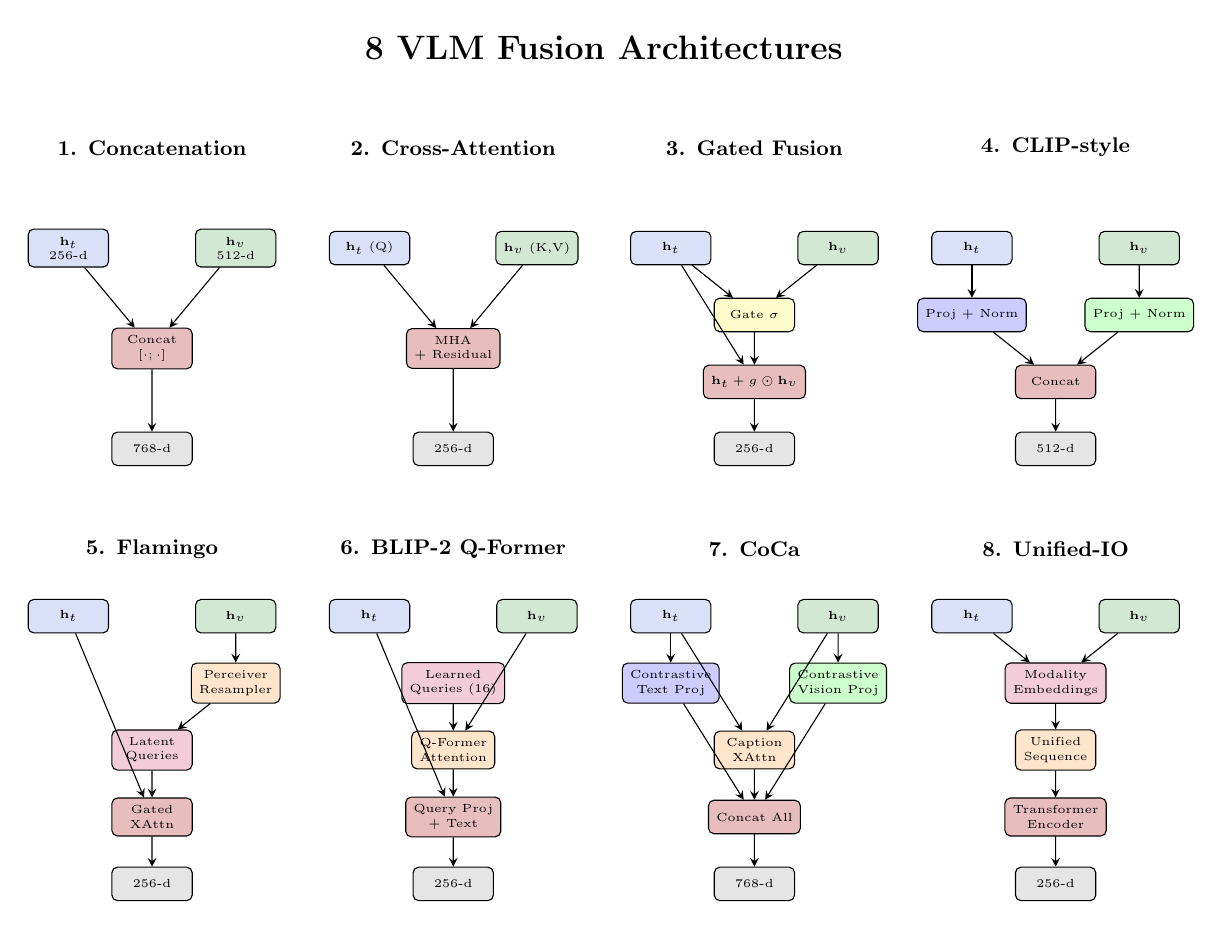
\begin{tikzpicture}[
    scale=0.85,
    transform shape,
    node distance=0.5cm,
    box/.style={rectangle, draw, rounded corners=2pt, minimum width=1.2cm, minimum height=0.5cm, align=center, font=\tiny},
    fusebox/.style={box, fill=vlmcolor!30},
    arrow/.style={->, >=stealth, font=\tiny}
]

% Title
\node[font=\Large\bfseries] at (8, 6) {8 VLM Fusion Architectures};

% ============ Row 1 ============

% 1. Concatenation
\begin{scope}[xshift=0cm]
    \node[font=\small\bfseries] at (1.25, 4.5) {1. Concatenation};
    \node[box, fill=llmcolor!20] (t1) at (0, 3) {$\mathbf{h}_t$\\256-d};
    \node[box, fill=vitcolor!20] (v1) at (2.5, 3) {$\mathbf{h}_v$\\512-d};
    \node[fusebox] (f1) at (1.25, 1.5) {Concat\\$[\cdot ; \cdot]$};
    \node[box, fill=gray!20] (o1) at (1.25, 0) {768-d};
    \draw[arrow] (t1) -- (f1);
    \draw[arrow] (v1) -- (f1);
    \draw[arrow] (f1) -- (o1);
\end{scope}

% 2. Cross-Attention
\begin{scope}[xshift=4.5cm]
    \node[font=\small\bfseries] at (1.25, 4.5) {2. Cross-Attention};
    \node[box, fill=llmcolor!20] (t2) at (0, 3) {$\mathbf{h}_t$ (Q)};
    \node[box, fill=vitcolor!20] (v2) at (2.5, 3) {$\mathbf{h}_v$ (K,V)};
    \node[fusebox] (f2) at (1.25, 1.5) {MHA\\+ Residual};
    \node[box, fill=gray!20] (o2) at (1.25, 0) {256-d};
    \draw[arrow] (t2) -- (f2);
    \draw[arrow] (v2) -- (f2);
    \draw[arrow] (f2) -- (o2);
\end{scope}

% 3. Gated Fusion
\begin{scope}[xshift=9cm]
    \node[font=\small\bfseries] at (1.25, 4.5) {3. Gated Fusion};
    \node[box, fill=llmcolor!20] (t3) at (0, 3) {$\mathbf{h}_t$};
    \node[box, fill=vitcolor!20] (v3) at (2.5, 3) {$\mathbf{h}_v$};
    \node[box, fill=yellow!20] (g3) at (1.25, 2) {Gate $\sigma$};
    \node[fusebox] (f3) at (1.25, 1) {$\mathbf{h}_t + g \odot \mathbf{h}_v$};
    \node[box, fill=gray!20] (o3) at (1.25, 0) {256-d};
    \draw[arrow] (t3) -- (g3);
    \draw[arrow] (v3) -- (g3);
    \draw[arrow] (t3) -- (f3);
    \draw[arrow] (g3) -- (f3);
    \draw[arrow] (f3) -- (o3);
\end{scope}

% 4. CLIP-style
\begin{scope}[xshift=13.5cm]
    \node[font=\small\bfseries] at (1.25, 4.5) {4. CLIP-style};
    \node[box, fill=llmcolor!20] (t4) at (0, 3) {$\mathbf{h}_t$};
    \node[box, fill=vitcolor!20] (v4) at (2.5, 3) {$\mathbf{h}_v$};
    \node[box, fill=blue!20] (p4a) at (0, 2) {Proj + Norm};
    \node[box, fill=green!20] (p4b) at (2.5, 2) {Proj + Norm};
    \node[fusebox] (f4) at (1.25, 1) {Concat};
    \node[box, fill=gray!20] (o4) at (1.25, 0) {512-d};
    \draw[arrow] (t4) -- (p4a);
    \draw[arrow] (v4) -- (p4b);
    \draw[arrow] (p4a) -- (f4);
    \draw[arrow] (p4b) -- (f4);
    \draw[arrow] (f4) -- (o4);
\end{scope}

% ============ Row 2 ============

% 5. Flamingo
\begin{scope}[xshift=0cm, yshift=-6cm]
    \node[font=\small\bfseries] at (1.25, 4.5) {5. Flamingo};
    \node[box, fill=llmcolor!20] (t5) at (0, 3.5) {$\mathbf{h}_t$};
    \node[box, fill=vitcolor!20] (v5) at (2.5, 3.5) {$\mathbf{h}_v$};
    \node[box, fill=orange!20] (perc) at (2.5, 2.5) {Perceiver\\Resampler};
    \node[box, fill=purple!20] (lat) at (1.25, 1.5) {Latent\\Queries};
    \node[fusebox] (f5) at (1.25, 0.5) {Gated\\XAttn};
    \node[box, fill=gray!20] (o5) at (1.25, -0.5) {256-d};
    \draw[arrow] (v5) -- (perc);
    \draw[arrow] (perc) -- (lat);
    \draw[arrow] (t5) -- (f5);
    \draw[arrow] (lat) -- (f5);
    \draw[arrow] (f5) -- (o5);
\end{scope}

% 6. BLIP-2
\begin{scope}[xshift=4.5cm, yshift=-6cm]
    \node[font=\small\bfseries] at (1.25, 4.5) {6. BLIP-2 Q-Former};
    \node[box, fill=llmcolor!20] (t6) at (0, 3.5) {$\mathbf{h}_t$};
    \node[box, fill=vitcolor!20] (v6) at (2.5, 3.5) {$\mathbf{h}_v$};
    \node[box, fill=purple!20] (q6) at (1.25, 2.5) {Learned\\Queries (16)};
    \node[box, fill=orange!20] (qf) at (1.25, 1.5) {Q-Former\\Attention};
    \node[fusebox] (f6) at (1.25, 0.5) {Query Proj\\+ Text};
    \node[box, fill=gray!20] (o6) at (1.25, -0.5) {256-d};
    \draw[arrow] (v6) -- (qf);
    \draw[arrow] (q6) -- (qf);
    \draw[arrow] (t6) -- (f6);
    \draw[arrow] (qf) -- (f6);
    \draw[arrow] (f6) -- (o6);
\end{scope}

% 7. CoCa
\begin{scope}[xshift=9cm, yshift=-6cm]
    \node[font=\small\bfseries] at (1.25, 4.5) {7. CoCa};
    \node[box, fill=llmcolor!20] (t7) at (0, 3.5) {$\mathbf{h}_t$};
    \node[box, fill=vitcolor!20] (v7) at (2.5, 3.5) {$\mathbf{h}_v$};
    \node[box, fill=blue!20] (ct) at (0, 2.5) {Contrastive\\Text Proj};
    \node[box, fill=green!20] (cv) at (2.5, 2.5) {Contrastive\\Vision Proj};
    \node[box, fill=orange!20] (cap) at (1.25, 1.5) {Caption\\XAttn};
    \node[fusebox] (f7) at (1.25, 0.5) {Concat All};
    \node[box, fill=gray!20] (o7) at (1.25, -0.5) {768-d};
    \draw[arrow] (t7) -- (ct);
    \draw[arrow] (v7) -- (cv);
    \draw[arrow] (t7) -- (cap);
    \draw[arrow] (v7) -- (cap);
    \draw[arrow] (ct) -- (f7);
    \draw[arrow] (cv) -- (f7);
    \draw[arrow] (cap) -- (f7);
    \draw[arrow] (f7) -- (o7);
\end{scope}

% 8. Unified-IO
\begin{scope}[xshift=13.5cm, yshift=-6cm]
    \node[font=\small\bfseries] at (1.25, 4.5) {8. Unified-IO};
    \node[box, fill=llmcolor!20] (t8) at (0, 3.5) {$\mathbf{h}_t$};
    \node[box, fill=vitcolor!20] (v8) at (2.5, 3.5) {$\mathbf{h}_v$};
    \node[box, fill=purple!20] (mod) at (1.25, 2.5) {Modality\\Embeddings};
    \node[box, fill=orange!20] (seq) at (1.25, 1.5) {Unified\\Sequence};
    \node[fusebox] (f8) at (1.25, 0.5) {Transformer\\Encoder};
    \node[box, fill=gray!20] (o8) at (1.25, -0.5) {256-d};
    \draw[arrow] (t8) -- (mod);
    \draw[arrow] (v8) -- (mod);
    \draw[arrow] (mod) -- (seq);
    \draw[arrow] (seq) -- (f8);
    \draw[arrow] (f8) -- (o8);
\end{scope}

\end{tikzpicture}

\newpage

% ============================================================================
% FIGURE 5: Federated Learning Architecture
% ============================================================================
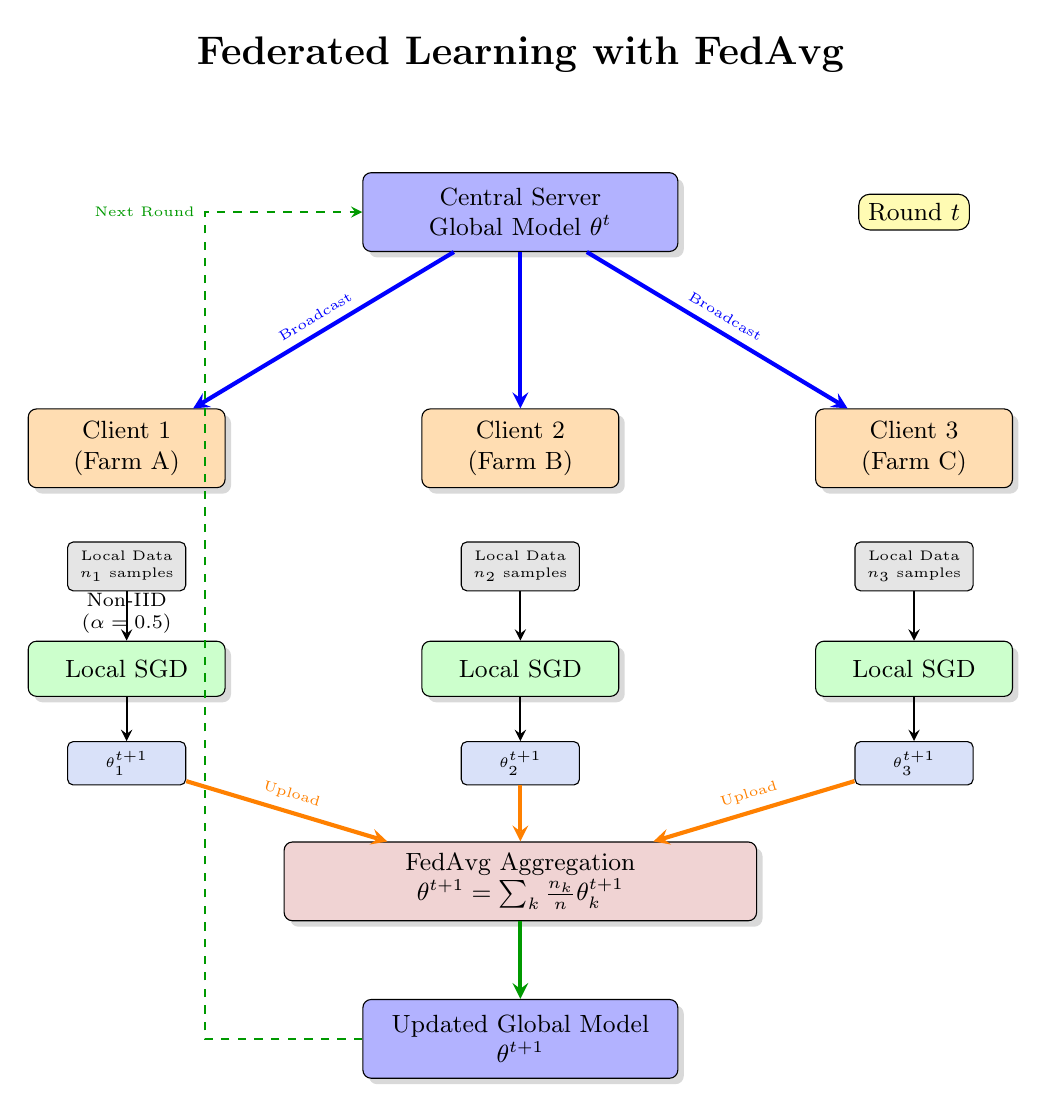
\begin{tikzpicture}[
    node distance=1.5cm,
    box/.style={rectangle, draw, rounded corners=3pt, minimum width=2.5cm, minimum height=1cm, align=center, font=\small, drop shadow={opacity=0.3}},
    clientbox/.style={box, fill=fedcolor!30},
    serverbox/.style={box, fill=blue!30},
    databox/.style={rectangle, draw, rounded corners=2pt, minimum width=1.5cm, minimum height=0.5cm, align=center, font=\tiny, fill=gray!20},
    arrow/.style={->, >=stealth, thick}
]

% Title
\node[font=\Large\bfseries] at (5, 7) {Federated Learning with FedAvg};

% Server
\node[serverbox, minimum width=4cm] (server) at (5, 5) {Central Server\\Global Model $\theta^t$};

% Round indicator
\node[font=\small, fill=yellow!30, draw, rounded corners] at (10, 5) {Round $t$};

% Clients
\node[clientbox] (c1) at (0, 2) {Client 1\\(Farm A)};
\node[clientbox] (c2) at (5, 2) {Client 2\\(Farm B)};
\node[clientbox] (c3) at (10, 2) {Client 3\\(Farm C)};

% Local data
\node[databox] (d1) at (0, 0.5) {Local Data\\$n_1$ samples};
\node[databox] (d2) at (5, 0.5) {Local Data\\$n_2$ samples};
\node[databox] (d3) at (10, 0.5) {Local Data\\$n_3$ samples};

% Local training
\node[box, fill=green!20, minimum height=0.7cm] (t1) at (0, -0.8) {Local SGD};
\node[box, fill=green!20, minimum height=0.7cm] (t2) at (5, -0.8) {Local SGD};
\node[box, fill=green!20, minimum height=0.7cm] (t3) at (10, -0.8) {Local SGD};

% Updated models
\node[databox, fill=llmcolor!20] (m1) at (0, -2) {$\theta_1^{t+1}$};
\node[databox, fill=llmcolor!20] (m2) at (5, -2) {$\theta_2^{t+1}$};
\node[databox, fill=llmcolor!20] (m3) at (10, -2) {$\theta_3^{t+1}$};

% Aggregation
\node[box, fill=vlmcolor!20, minimum width=6cm] (agg) at (5, -3.5) {FedAvg Aggregation\\$\theta^{t+1} = \sum_k \frac{n_k}{n} \theta_k^{t+1}$};

% New global model
\node[serverbox, minimum width=4cm] (newserver) at (5, -5.5) {Updated Global Model\\$\theta^{t+1}$};

% Arrows - broadcast
\draw[arrow, blue, line width=1.5pt] (server) -- (c1) node[midway, above, sloped, font=\tiny] {Broadcast};
\draw[arrow, blue, line width=1.5pt] (server) -- (c2);
\draw[arrow, blue, line width=1.5pt] (server) -- (c3) node[midway, above, sloped, font=\tiny] {Broadcast};

% Arrows - data to training
\draw[arrow] (d1) -- (t1);
\draw[arrow] (d2) -- (t2);
\draw[arrow] (d3) -- (t3);

% Arrows - training to models
\draw[arrow] (t1) -- (m1);
\draw[arrow] (t2) -- (m2);
\draw[arrow] (t3) -- (m3);

% Arrows - models to aggregation
\draw[arrow, orange, line width=1.5pt] (m1) -- (agg) node[midway, above, sloped, font=\tiny] {Upload};
\draw[arrow, orange, line width=1.5pt] (m2) -- (agg);
\draw[arrow, orange, line width=1.5pt] (m3) -- (agg) node[midway, above, sloped, font=\tiny] {Upload};

% Arrow - aggregation to new server
\draw[arrow, green!60!black, line width=1.5pt] (agg) -- (newserver);

% Loop back
\draw[arrow, dashed, green!60!black] (newserver.west) -- ++(-2,0) |- (server.west) node[midway, left, font=\tiny] {Next Round};

% Non-IID annotation
\node[font=\scriptsize, align=center] at (0, -0.1) {Non-IID\\($\alpha = 0.5$)};

\end{tikzpicture}

\newpage

% ============================================================================
% FIGURE 6: Class Imbalance Handling
% ============================================================================
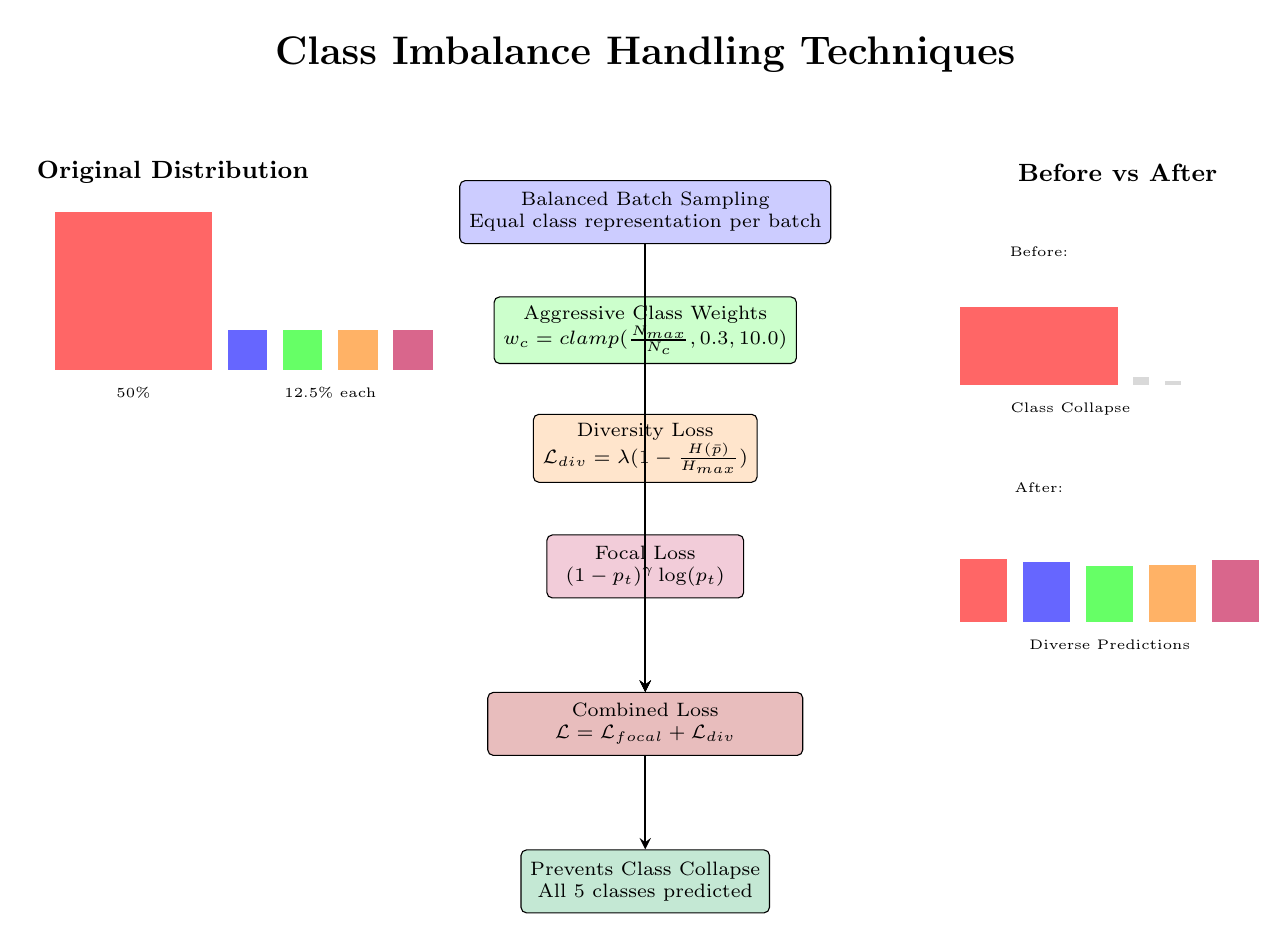
\begin{tikzpicture}[
    node distance=1cm,
    box/.style={rectangle, draw, rounded corners=2pt, minimum width=2.5cm, minimum height=0.8cm, align=center, font=\scriptsize},
    arrow/.style={->, >=stealth, thick}
]

% Title
\node[font=\Large\bfseries] at (6, 7) {Class Imbalance Handling Techniques};

% Original distribution
\node[font=\small\bfseries] at (0, 5.5) {Original Distribution};
\begin{scope}[xshift=-1.5cm, yshift=3cm]
    \fill[red!60] (0,0) rectangle (2, 2);
    \fill[blue!60] (2.2,0) rectangle (2.7, 0.5);
    \fill[green!60] (2.9,0) rectangle (3.4, 0.5);
    \fill[orange!60] (3.6,0) rectangle (4.1, 0.5);
    \fill[purple!60] (4.3,0) rectangle (4.8, 0.5);
    \node[font=\tiny] at (1, -0.3) {50\%};
    \node[font=\tiny] at (3.5, -0.3) {12.5\% each};
\end{scope}

% Technique 1: Balanced Sampling
\node[box, fill=blue!20] (bs) at (6, 5) {Balanced Batch Sampling\\Equal class representation per batch};

% Technique 2: Class Weights
\node[box, fill=green!20] (cw) at (6, 3.5) {Aggressive Class Weights\\$w_c = \text{clamp}(\frac{N_{max}}{N_c}, 0.3, 10.0)$};

% Technique 3: Diversity Loss
\node[box, fill=orange!20] (dl) at (6, 2) {Diversity Loss\\$\mathcal{L}_{div} = \lambda(1 - \frac{H(\bar{p})}{H_{max}})$};

% Technique 4: Focal Loss
\node[box, fill=purple!20] (fl) at (6, 0.5) {Focal Loss\\$(1-p_t)^\gamma \log(p_t)$};

% Combined
\node[box, fill=vlmcolor!30, minimum width=4cm] (combined) at (6, -1.5) {Combined Loss\\$\mathcal{L} = \mathcal{L}_{focal} + \mathcal{L}_{div}$};

% Arrows
\draw[arrow] (bs) -- (combined);
\draw[arrow] (cw) -- (combined);
\draw[arrow] (dl) -- (combined);
\draw[arrow] (fl) -- (combined);

% Result
\node[box, fill=outputcolor!30] (result) at (6, -3.5) {Prevents Class Collapse\\All 5 classes predicted};

\draw[arrow] (combined) -- (result);

% Before/After visualization
\node[font=\small\bfseries] at (12, 5.5) {Before vs After};

% Before
\node[font=\tiny] at (11, 4.5) {Before:};
\begin{scope}[xshift=10cm, yshift=2.8cm]
    \fill[red!60] (0,0) rectangle (2, 1);
    \fill[gray!30] (2.2,0) rectangle (2.4, 0.1);
    \fill[gray!30] (2.6,0) rectangle (2.8, 0.05);
    \node[font=\tiny] at (1.4, -0.3) {Class Collapse};
\end{scope}

% After
\node[font=\tiny] at (11, 1.5) {After:};
\begin{scope}[xshift=10cm, yshift=-0.2cm]
    \fill[red!60] (0,0) rectangle (0.6, 0.8);
    \fill[blue!60] (0.8,0) rectangle (1.4, 0.75);
    \fill[green!60] (1.6,0) rectangle (2.2, 0.7);
    \fill[orange!60] (2.4,0) rectangle (3.0, 0.72);
    \fill[purple!60] (3.2,0) rectangle (3.8, 0.78);
    \node[font=\tiny] at (1.9, -0.3) {Diverse Predictions};
\end{scope}

\end{tikzpicture}

\newpage

% ============================================================================
% FIGURE 7: Qdrant Semantic Retrieval
% ============================================================================
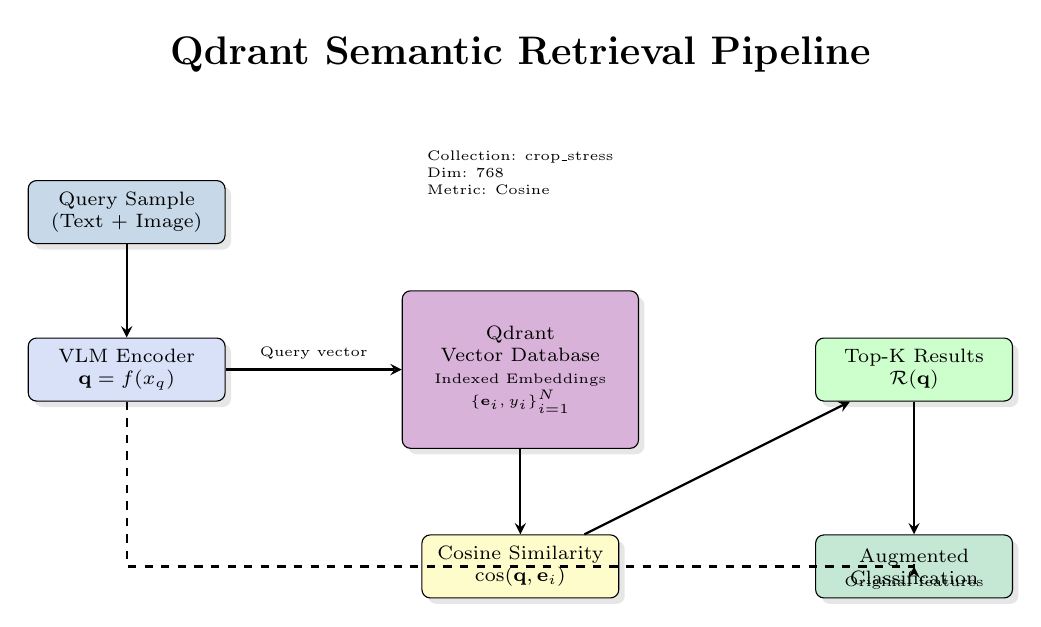
\begin{tikzpicture}[
    node distance=1cm,
    box/.style={rectangle, draw, rounded corners=3pt, minimum width=2.5cm, minimum height=0.8cm, align=center, font=\scriptsize, drop shadow={opacity=0.2}},
    arrow/.style={->, >=stealth, thick}
]

% Title
\node[font=\Large\bfseries] at (5, 6) {Qdrant Semantic Retrieval Pipeline};

% Query input
\node[box, fill=inputcolor!30] (query) at (0, 4) {Query Sample\\(Text + Image)};

% Encoder
\node[box, fill=llmcolor!20] (enc) at (0, 2) {VLM Encoder\\$\mathbf{q} = f(x_q)$};

% Qdrant DB
\node[box, fill=qdrantcolor!30, minimum width=3cm, minimum height=2cm] (qdrant) at (5, 2) {Qdrant\\Vector Database\\{\tiny Indexed Embeddings}\\{\tiny $\{\mathbf{e}_i, y_i\}_{i=1}^N$}};

% Similarity search
\node[box, fill=yellow!20] (search) at (5, -0.5) {Cosine Similarity\\$\cos(\mathbf{q}, \mathbf{e}_i)$};

% Top-k results
\node[box, fill=green!20] (topk) at (10, 2) {Top-K Results\\$\mathcal{R}(\mathbf{q})$};

% Augmented prediction
\node[box, fill=outputcolor!30] (pred) at (10, -0.5) {Augmented\\Classification};

% Arrows
\draw[arrow] (query) -- (enc);
\draw[arrow] (enc) -- (qdrant) node[midway, above, font=\tiny] {Query vector};
\draw[arrow] (qdrant) -- (search);
\draw[arrow] (search) -- (topk);
\draw[arrow] (topk) -- (pred);
\draw[arrow, dashed] (enc) -- ++(0, -2.5) -| (pred) node[midway, below, font=\tiny] {Original features};

% Collection info
\node[font=\tiny, align=left] at (5, 4.5) {Collection: crop\_stress\\Dim: 768\\Metric: Cosine};

\end{tikzpicture}

\end{document}
